\documentclass{article}

\usepackage[UTF8]{ctex}
\usepackage{placeins}
\usepackage{graphicx}
\usepackage{listings}
\usepackage{xcolor} % 添加 xcolor 宏包
\lstset{ %
language=matlab,                % choose the language of the code
basicstyle=\footnotesize,       % the size of the fonts that are used for the code
numbers=left,                   % where to put the line-numbers
numberstyle=\footnotesize,      % the size of the fonts that are used for the line-numbers
stepnumber=1,                   % the step between two line-numbers. If it is 1 each line will be numbered
numbersep=5pt,                  % how far the line-numbers are from the code
backgroundcolor=\color{white},  % choose the background color. You must add \usepackage{color}
showspaces=false,               % show spaces adding particular underscores
showstringspaces=false,         % underline spaces within strings
showtabs=false,                 % show tabs within strings adding particular underscores
frame=single,           % adds a frame around the code
tabsize=2,          % sets default tabsize to 2 spaces
captionpos=b,           % sets the caption-position to bottom
breaklines=true,        % sets automatic line breaking
breakatwhitespace=false,    % sets if automatic breaks should only happen at whitespace
escapeinside={\%*}{*)}          % if you want to add a comment within your code
}
\title{hw02\_MATLAB}
\author{3220103167 缪晨轩}
\date{\zhdate{2024/3/4}}

\begin{document}

\maketitle

    \section*{58(1)}
        \begin{lstlisting}[caption={题58(1)MATLAB代码}, label={lst:matlab}]
            syms t T;

            % 原始信号 sin(t)
            original_signal = sin(t);

            % 向右平移了T/2的冲激信号
            shifted_signal = dirac(t - T/2);

            % 计算乘积
            product_signal = original_signal * shifted_signal;

            % 计算在(-∞, ∞)上的积分
            integral_product = int(product_signal, t, -inf, inf);

            disp(['sin(t) 与向右平移了T/2的冲激信号乘积在(-∞, ∞)上的积分: ', char(integral_product)]);

        \end{lstlisting}
        Answer: \[\sin \left( {\frac{{{T_1}}}{2}} \right)\]
    \section*{58(2)}
        \begin{lstlisting}[caption={题58(2)MATLAB代码}, label={lst:matlab}]
            syms t;

            % 信号1
            coefficients = [1, 0, 1, 2];
            polynomial_value = poly2sym(coefficients, t);

            % 信号2
            shifted_dirac = dirac(t - 1);

            % 计算抽样值
            integral_product = int(polynomial_value * shifted_dirac, t, -inf, inf);

            fprintf('抽样结果:%s\n', char(integral_product));

        \end{lstlisting}
        Answer: 4
    \section*{Additional(2)(1)}
        \begin{lstlisting}[caption={题Additional(2)(1)MATLAB代码}, label={lst:matlab}]
            t1 = 0:0.01:1; % 时间范围从0到1,采样间隔0.01
            x1 = ones(size(t1)); % 信号值为1

            t2 = 1:0.01:2; % 时间范围从1到2,采样间隔0.01
            x2 = zeros(size(t2)); % 信号值为0

            t = [t1 t2]; % 合并时间向量
            x = [x1 x2]; % 合并信号值向量

            y = conv(x, x, 'same'); % 计算信号x与自身的卷积

            subplot(2,1,1);
            plot(t, x);
            title('Original Signal');
            xlabel('Time');
            ylabel('Amplitude');

            subplot(2,1,2);
            plot(t, y);
            title('Convolved Signal');
            xlabel('Time');
            ylabel('Amplitude');

        \end{lstlisting}
        Answer: 
            \begin{figure}[h]
                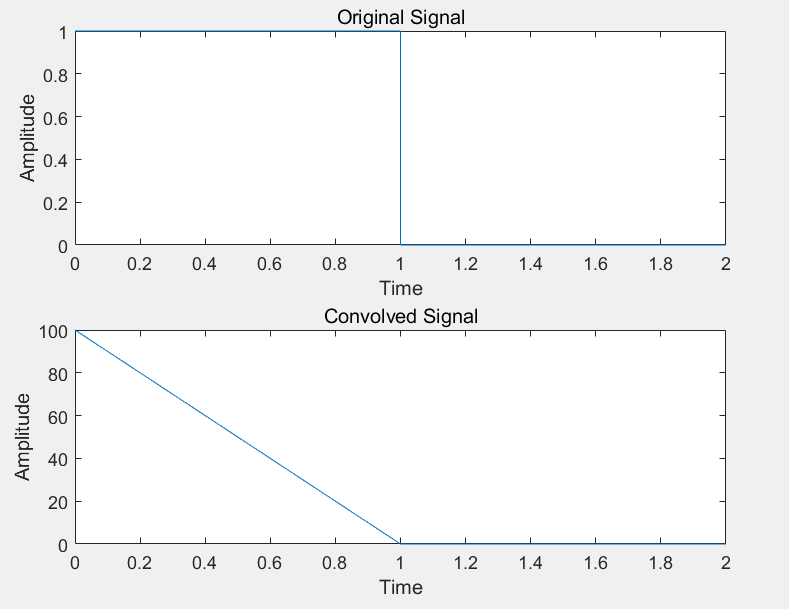
\includegraphics{additional_1.png}
            \end{figure}
            \FloatBarrier
    \section*{Addition(2)(2)}
        \begin{lstlisting}[caption={题Additional(2)(2)MATLAB代码}, label={lst:matlab}]
            % 定义时间向量
            t = 0:0.01:2;

            % 信号一:在0时刻突变为1,之后保持1直到1时刻突变为0
            signal_1 = zeros(size(t));
            signal_1(t >= 0 & t < 1) = 1;

            % 信号二:在0时刻突变为1,然后线性下降至1时刻为0
            signal_2 = zeros(size(t));
            signal_2(t >= 0 & t < 1) = 1 - t(t >= 0 & t < 1);

            % 计算卷积
            convolution_result = conv(signal_1, signal_2, 'full');

            % 绘制信号和卷积结果
            figure;

            subplot(3,1,1);
            plot(t, signal_1);
            title('信号一');

            subplot(3,1,2);
            plot(t, signal_2);
            title('信号二');

            subplot(3,1,3);
            t_conv = 0:0.01:4; % 卷积结果的时间范围
            plot(t_conv, convolution_result);
            title('信号一和信号二的卷积结果');
            xlabel('时间');


        \end{lstlisting}
        Answer: 
            \begin{figure}[h]
                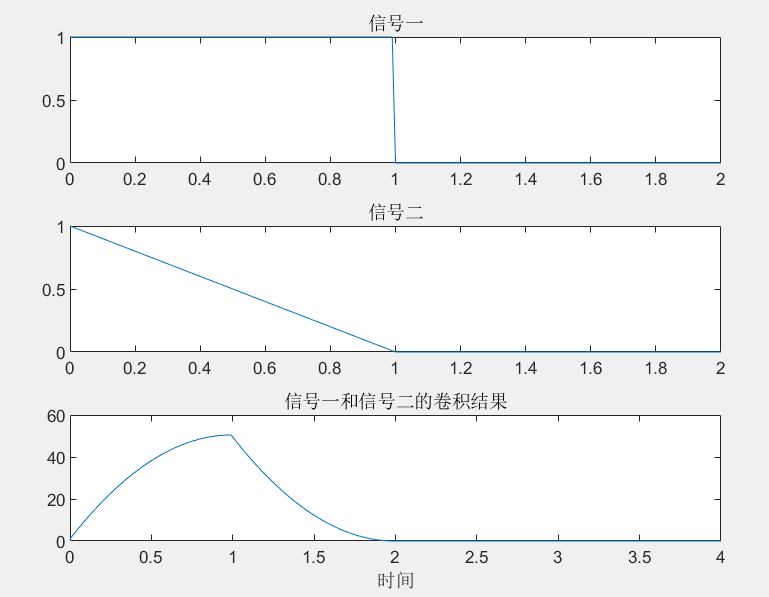
\includegraphics{additional_2.png}
            \end{figure}
            \FloatBarrier
\end{document}